\begin{figure*}
\centering

%%%%%%%%% ----- Map ------- %%%%%
\newsavebox{\MapHLL}
\begin{lrbox}{\MapHLL}
\begin{lstlisting}[language=PPLTable]
// Vector multiplied by 2
vector * 2

// Addition of two vectors
vectorA + vectorB
\end{lstlisting}
\end{lrbox}

\newsavebox{\MapPPL}
\begin{lrbox}{\MapPPL}
\begin{lstlisting}[language=PPLTable]

Map(s){i => vector(i) * 2 }


Map(s){i =>
  vectorA(i) + vectorB(i)
}
\end{lstlisting}
\end{lrbox}

%%%%%%%%% ----- MultiFold ------- %%%%%
\newsavebox{\MultiFoldHLLOne}
\begin{lrbox}{\MultiFoldHLLOne}
\begin{lstlisting}[language=PPLTable]
// Product of a size s vector
vector.sum

\end{lstlisting}
\end{lrbox}

\newsavebox{\MultiFoldHLLTwo}
\begin{lrbox}{\MultiFoldHLLTwo}
\begin{lstlisting}[language=PPLTable]
// Row sums in an s $\times$ t matrix
x.mapRows{row => row.sum }

\end{lstlisting}
\end{lrbox}

\newsavebox{\MultiFoldPPLOne}
\begin{lrbox}{\MultiFoldPPLOne}
\begin{lstlisting}[language=PPLTable]
MultiFold(s)(1)(1){ i =>
  (0, acc => acc + vector(i))
}{ (a,b) => a + b }
\end{lstlisting}
\end{lrbox}

\newsavebox{\MultiFoldPPLTwo}
\begin{lrbox}{\MultiFoldPPLTwo}
\begin{lstlisting}[language=PPLTable]
MultiFold(s,t)(r)(zeros(s))
{ (i,j) =>
  (i, acc => acc + x(i,j) )
}{ (a,b) =>
  Map(s){ i => a(i) + b(i) }
}
\end{lstlisting}
\end{lrbox}

%%%%%%%%% ----- FlatMap ------- %%%%%
\newsavebox{\FlatMapHLL}
\begin{lrbox}{\FlatMapHLL}
\begin{lstlisting}[language=PPLTable]
// Filter positive values
SELECT * FROM vector
  WHERE elem >= 0

\end{lstlisting}
\end{lrbox}

\newsavebox{\FlatMapPPL}
\begin{lrbox}{\FlatMapPPL}
\begin{lstlisting}[language=PPLTable]
FlatMap(s){ i =>
  if (x(i) > 0) [x(i)] else []
}

\end{lstlisting}
\end{lrbox}

%%%%%%%%% ----- GroupByFold ------- %%%%%
\newsavebox{\GroupByFoldHLL}
\begin{lrbox}{\GroupByFoldHLL}
\begin{lstlisting}[language=PPLTable]
// Histogram, bin width 10
x.groupByFold(0){ e =>
  (e/10, 1)
}{ (a,b) => a + b }
\end{lstlisting}
\end{lrbox}

\newsavebox{\GroupByFoldPPL}
\begin{lrbox}{\GroupByFoldPPL}
\begin{lstlisting}[language=PPLTable]
GroupByFold(s)(0){ i =>
  (x(i)/10, acc => acc + 1)
}{ (a,b) => a + b }

\end{lstlisting}
\end{lrbox}

\resizebox{\textwidth}{!}{%% begin resizebox
\begin{tabular}{lll}
\textbf{Visual Example} & \textbf{DSL Example} & \textbf{PPL Representation} \\
\hline\hline

{\begin{tabular}{c}
  \texttt{\footnotesize{Indices}}\vspace{-6pt} \\
  \vspace{-0.5mm}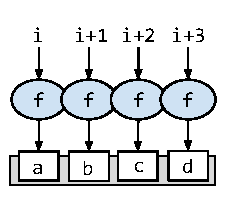
\includegraphics[width=2.6cm]{2-background/figs/Map} \\
  \texttt{\footnotesize{\textbf{Map}}} \\
\end{tabular}}
& \usebox{\MapHLL}
& \usebox{\MapPPL} \\ \hline
\vspace{-6pt} & & \\

\multirow{4}{*}{
\begin{tabular}{c}
  \vspace{-30pt} \\
  \texttt{\footnotesize{Indices}}\vspace{-6pt} \\
  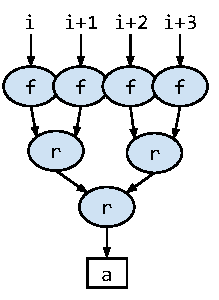
\includegraphics[width=2.6cm]{2-background/figs/Reduce} \\
  \texttt{\footnotesize{\textbf{MultiFold}}} \\
\end{tabular}\vspace{12pt}}
&
{\hspace{-6pt}\begin{tabular}{l}
\usebox{\MultiFoldHLLOne}  \\  \\
\end{tabular}}
& \usebox{\MultiFoldPPLOne} \\
\vspace{-6pt} & & \\
&
{\hspace{-6pt}\begin{tabular}{l}
\usebox{\MultiFoldHLLTwo} \\ \\ \\ \\
\end{tabular}}
& \usebox{\MultiFoldPPLTwo} \\
& & \\ \hline
\vspace{-6pt} & & \\

{\begin{tabular}{c}
  \texttt{\footnotesize{ Indices}}\vspace{-6pt} \\
  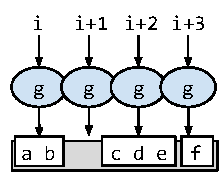
\includegraphics[width=2.6cm]{2-background/figs/FlatMap} \\
  \texttt{\footnotesize{\textbf{FlatMap}}} \\
\end{tabular}}
& \usebox{\FlatMapHLL}
& \usebox{\FlatMapPPL} \\ \hline
\vspace{-6pt} & & \\

{\begin{tabular}{c}
  \texttt{\footnotesize{  Indices}}\vspace{-6pt} \\
  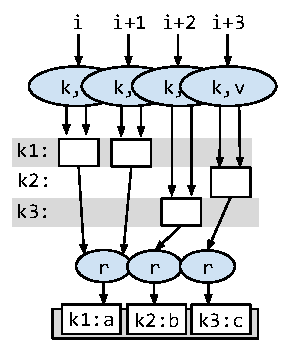
\includegraphics[width=3.2cm]{2-background/figs/HashReduce} \\
  \texttt{\footnotesize{\textbf{GroupByFold}}} \\
\end{tabular}}
& \usebox{\GroupByFoldHLL}
& \usebox{\GroupByFoldPPL} \\
\end{tabular} %% end resizebox
} %% end resizebox

\caption{\label{fig:ppl-examples}Usage examples for patterns in the PPL from various domain-specific languages.}
\end{figure*}
